\documentclass{article} % Change to a standard article class
\usepackage{amsmath} % for math environments and commands
\usepackage{cite}
\usepackage{amssymb}
\usepackage{amsfonts}
\usepackage{graphicx}
\usepackage{textcomp}
\usepackage{xcolor}
\usepackage{amsmath}


\begin{document}

\title{K Nearest Neighbors part 2\\
\thanks{Insert applicable funding agency here. If none, delete this.}
}

\author{Arthur Felipe Reis Souza \\
Electrical Engineering Department, \\
Federal University of Minas Gerais, \\
Belo Horizonte, Brazil \\
arthurfreisouza@gmail.com \\
\and
Antônio de Pádua Braga and Frederico Gualberto Ferreira Coelho \\
Electrical Engineering Department, \\
Federal University of Minas Gerais, \\
Belo Horizonte, Brazil \\
apbraga@cpdee.ufmg.br, fredgfc@ufmg.br
}

\maketitle

\begin{abstract}

    A primeira parte desse relatório visa demonstrar a performance do KNN, em 1 dataset real obtido no Kaggle, ao variar o parâmetro K. A segunda parte consiste em estudar como os pontos são mapeados em um novo espaço através de uma função Gaussiana de Kernel.

\end{abstract}

\newpage

\section{Parte 1}

\subsection{Introdução}

O KNN (K-Nearest Neighbors) é um algoritmo de Machine Learning utilizado para tarefas de classificação e regressão. Neste trabalho, uma base de dados obtida no Kaggle foi utilizada para testar o KNN como classificador. Essa base contém informações detalhadas sobre pacientes, e a classificação final é realizada com base nessas características. O resultado da classificação será -1, indicando uma baixa probabilidade de o paciente sofrer um ataque cardíaco, ou 1, sinalizando uma alta probabilidade de ocorrência.

\vspace{1cm}

A figura abaixo mostra a base de dados, a qual as colunas indicam as características do paciente, enquanto as linhas indicam cada paciente : 

\vspace{1cm}

\begin{figure}[h] % 'h' posiciona a figura aproximadamente no local do código
    \centering % centraliza a figura
    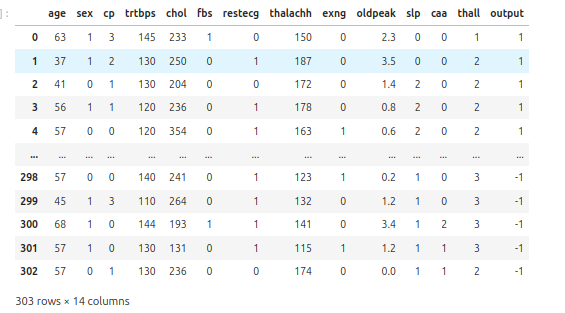
\includegraphics[width=1\linewidth]{dataset.png} % insira o caminho da sua imagem e ajuste a largura
    \caption{Algoritmo KNN.} % insira a legenda desejada
    \label{fig:exemplo} % rótulo para referenciar a figura no texto
\end{figure}

\vspace{1cm}

Portanto, espera-se que com base nas características de cada paciente, o modelo realize uma previsão se o mesmo terá ou não um ataque cardíaco futuramente.

\newpage

\subsection{Pré Processamento dos dados}

Durante o pré-processamento, inicialmente foram realizados estudos de correlação entre as variáveis da base de dados. Isso porque características com alta correlação podem causar problemas de multicolinearidade (forte correlação entre duas ou mais variáveis), o que pode comprometer o desempenho do classificador. Após essa análise, foi aplicada uma técnica de normalização para garantir que todas as variáveis estivessem na mesma escala, variando de 0 a 1. Essa etapa é fundamental, pois o KNN é um algoritmo sensível a distâncias, e variáveis em escalas diferentes resultariam em um desempenho insatisfatório. Por fim, utilizou-se a função train test split do Python para dividir os dados em conjunto de treino e teste, 85\% dos dados para o treinamento e 15\% para a inferência (teste).

\vspace{1cm}

A imagem abaixo contém a matriz de correlação dos dados : 

\vspace{1cm}

\begin{figure}[h] % 'h' posiciona a figura aproximadamente no local do código
    \centering % centraliza a figura
    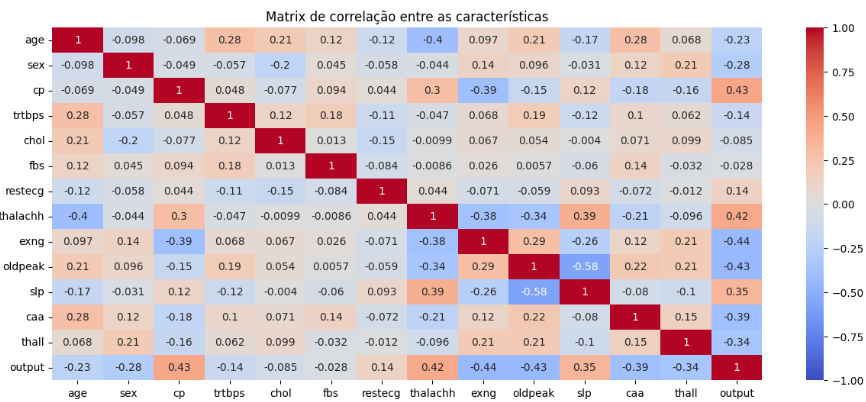
\includegraphics[width=1\linewidth]{corr_matrix.png} % insira o caminho da sua imagem e ajuste a largura
    \caption{Matriz de correlação da base de dados.} % insira a legenda desejada
    \label{fig:exemplo} % rótulo para referenciar a figura no texto
\end{figure}

\newpage

\subsection{Treinamento e resultados}

Após a divisão dos dados em conjuntos de treino e teste, o algoritmo KNN implementado no exercício anterior foi treinado utilizando o conjunto de treino. Esperava-se que o modelo apresentasse um bom desempenho durante a fase de inferência. Para aumentar a confiabilidade do modelo, foi realizada uma validação cruzada (Cross-Validation) para cada valor de K testado em um Grid que varia de 1 até 50. Em outras palavras, para cada valor de K, foram realizados 10 testes distintos, variando os dados de treino e teste a cada execução. A média dos resultados desses 10 testes, bem como o desvio padrão para cada valor de K, foram registrados em uma tabela. Esse método é eficaz porque aumenta a robustez do modelo e a sua confiabilidade, evitando que a presença de dados enviesados comprometa o desempenho do algoritmo.

\vspace{1cm}

A imagem abaixo mostra o resultado de apenas uma pequena parcela dos resultados da acurácia do modelo e o seu desvio padrão ao variar o parâmetro K em um Grid : 

\vspace{1cm}

\begin{figure}[h] % 'h' posiciona a figura aproximadamente no local do código
    \centering % centraliza a figura
    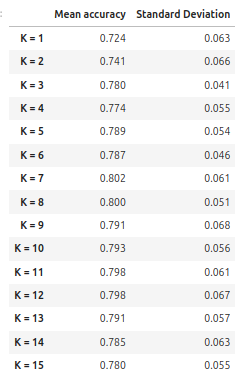
\includegraphics[width=0.5\linewidth]{table_k.png} % insira o caminho da sua imagem e ajuste a largura
    \caption{Tabela das acurácias.} % insira a legenda desejada
    \label{fig:exemplo} % rótulo para referenciar a figura no texto
\end{figure}

\vspace{1cm}

Como se pode reparar, ao variar o valor de K a performance do modelo também tende a se alterar. Para se ter uma noção melhor dessa variação, foi plotado um gráfico da variação da acurácia em função do número de Neighbors K, esse gráfico está plotado abaixo :

\vspace{1cm}

\begin{figure}[h] % 'h' posiciona a figura aproximadamente no local do código
    \centering % centraliza a figura
    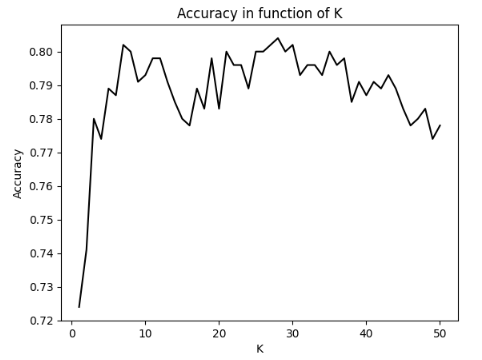
\includegraphics[width=1\linewidth]{graphic_k.png} % insira o caminho da sua imagem e ajuste a largura
    \caption{Gráfico da acurácia em função de K.} % insira a legenda desejada
    \label{fig:exemplo} % rótulo para referenciar a figura no texto
\end{figure}

\vspace{1cm}

A análise da figura demonstra que a acurácia do modelo inicialmente é baixa e aumenta com o aumento de K, atingindo um pico em K = 7, seguido de uma queda. Embora a acurácia suba novamente após K = 10, ela eventualmente declina rapidamente, tendendo a um valor baixo e constante conforme K se aproxima do infinito. Isso sugere que valores altos de K tornam o modelo menos eficaz, com a melhor performance alcançada em K = 7. É relevante notar que, apesar do aumento de acurácia após o primeiro declínio, a escolha de um K elevado não é ideal, pois resulta em maior consumo de recursos computacionais sem melhorias significativas. Portanto, uma abordagem recomendável para determinar o valor de K é realizar testes utilizando o algoritmo Grid-Search, visando selecionar o menor K que proporcione a melhor performance.

\newpage

\section{Parte 2}

\subsection{Discussão}

\vspace{1cm}

A segunda parte do exercício consiste em analisar o comportamento do classificador em um espaço de verossimilhanças. Basicamente, o KNN ponderado irá mapear os K vizinhos mais próximos da amostra a ser classificada em um novo espaço descrito pela equação:

\[
\hat{y} = \operatorname{sinal}\left(\sum_{i=1}^{k_1} K(x, x_i) - \sum_{j=1}^{k_2} K(x, x_j)\right)
\]

Esse mapeamento se dá por uma função de Kernel \( K(x_i, x_j) \) que é tipicamente Gaussiana. Após esse mapeamento dos K vizinhos mais próximos, a amostra será classificada dependendo do sinal resultante no somatório. A equação acima pode ser descrita, para cada amostra, como na equação abaixo : 

\[
\hat{y} = \operatorname{sinal}(Q_1(x|C_1) - Q_2(x|C_2))
\]

Inicialmente, é importante destacar dois aspectos: ao escolher um valor de K muito pequeno, os pontos tendem a se concentrar em um único eixo, seja Q2 ou Q1, já que apenas um termo do somatório será considerado. Por outro lado, ao optar por um valor de K muito elevado, os pontos provavelmente não sofrerão alterações no gráfico do espaço de verossimilhanças, uma vez que todos os pontos do conjunto de treino já estarão sendo empregados. 

\vspace{1cm}

Analisando os gráficos do espaço de verossimilhanças com a variação do valor de K, conclui-se que, ao aumentar K, os pontos (Q1,Q2) no gráfico são alterados. A localização de cada ponto no espaço de verossimilhanças depende do novo ponto cujas distâncias estão sendo medidas, pois a função de kernel leva os dados a esse novo espaço em relação a esse ponto. Um aspecto interessante é que, ao definir um valor par para K, as amostras se alinham sobre a reta que separa as classes, dificultando a classificação como positivas ou negativas. Por esse motivo, é necessário que K seja sempre um número ímpar. Além disso, quando K se torna muito grande, como observado para K = 300 e K = 10.000, os pontos no gráfico não se alteram, indicando que todos os pontos do conjunto de treino foram utilizados, o que não contribui para o somatório que influencia a classificação do novo ponto. A estratégia para K segue a mesma lógica do exercíco anterior.

\newpage

\begin{figure}[h] % 'h' posiciona a figura aproximadamente no local do código
    \centering % centraliza a figura
    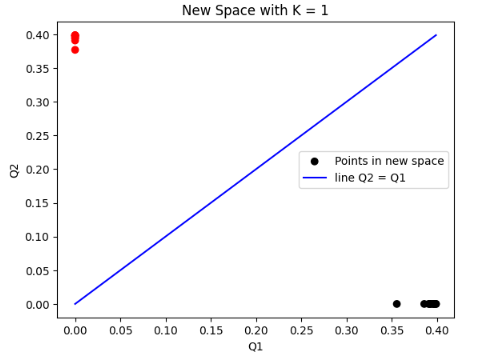
\includegraphics[width=1\linewidth]{k1.png} % insira o caminho da sua imagem e ajuste a largura
    \caption{Espaço de verossimilhanças com K = 1.} % insira a legenda desejada
    \label{fig:exemplo} % rótulo para referenciar a figura no texto
\end{figure}

\begin{figure}[h] % 'h' posiciona a figura aproximadamente no local do código
    \centering % centraliza a figura
    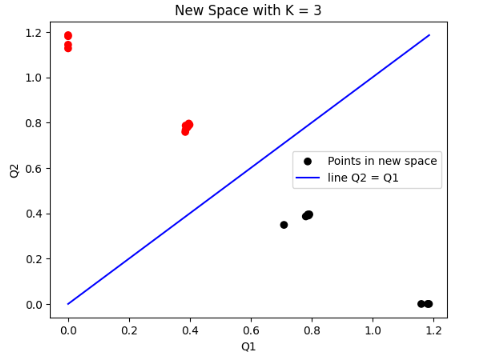
\includegraphics[width=1\linewidth]{k3.png} % insira o caminho da sua imagem e ajuste a largura
    \caption{Espaço de verossimilhanças com K = 3.} % insira a legenda desejada
    \label{fig:exemplo} % rótulo para referenciar a figura no texto
\end{figure}

\begin{figure}[h] % 'h' posiciona a figura aproximadamente no local do código
    \centering % centraliza a figura
    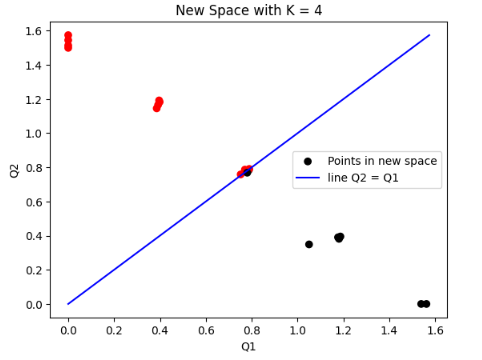
\includegraphics[width=1\linewidth]{k4.png} % insira o caminho da sua imagem e ajuste a largura
    \caption{Espaço de verossimilhanças com K = 4.} % insira a legenda desejada
    \label{fig:exemplo} % rótulo para referenciar a figura no texto
\end{figure}

\begin{figure}[h] % 'h' posiciona a figura aproximadamente no local do código
    \centering % centraliza a figura
    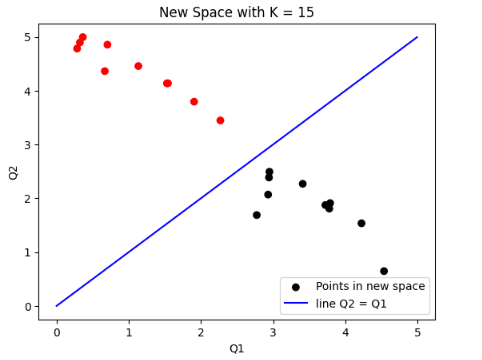
\includegraphics[width=1\linewidth]{k15.png} % insira o caminho da sua imagem e ajuste a largura
    \caption{Espaço de verossimilhanças com K = 15} % insira a legenda desejada
    \label{fig:exemplo} % rótulo para referenciar a figura no texto
\end{figure}

\begin{figure}[h] % 'h' posiciona a figura aproximadamente no local do código
    \centering % centraliza a figura
    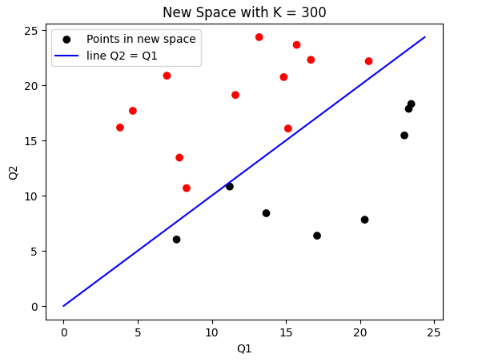
\includegraphics[width=1\linewidth]{k300.png} % insira o caminho da sua imagem e ajuste a largura
    \caption{Espaço de verossimilhanças com K = 300.} % insira a legenda desejada
    \label{fig:exemplo} % rótulo para referenciar a figura no texto
\end{figure}

\begin{figure}[h] % 'h' posiciona a figura aproximadamente no local do código
    \centering % centraliza a figura
    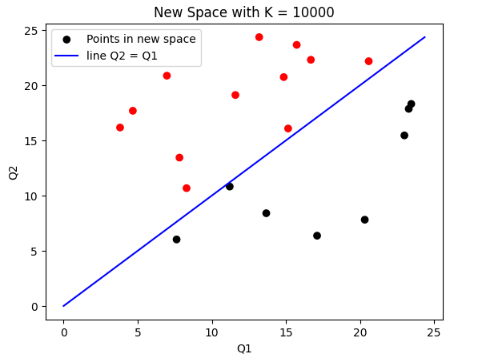
\includegraphics[width=1\linewidth]{k10000.png} % insira o caminho da sua imagem e ajuste a largura
    \caption{Espaço de verossimilhanças com K = 10000.} % insira a legenda desejada
    \label{fig:exemplo} % rótulo para referenciar a figura no texto
\end{figure}

\subsection{Conclusão}

Por fim, vale ressaltar que os objetivos do relatório foram concluídos, uma estratégia para encontrar o valor de K foi posta (Método Grid-Search, com foco no menor valor de K que gerará uma melhor performance), e também o estudo do espaço de verossimilhanças, o qual é alterado para cada valor de K.

\end{document}